\documentclass[twocolumn]{article}

\title{Orientation and design of LPC1769 CAN Bootloader}
\author{Chiel de Roest\\4036832 \and Harmjan Treep\\4011724}
\date{}

\usepackage[english]{babel}
\usepackage[pdfborder={0 0 0},plainpages=false]{hyperref}
\usepackage{fullpage}
\usepackage{graphicx}

% Hack to create memory diagrams inspired by http://www.martin-demling.de/2011/06/memory-maps-in-latex-using-the-bytefield-package/
\usepackage{bytefield}
\newcommand{\memsection}[4]{
	%\bytefieldsetup{bitheight=#3\baselineskip}    % define the height of the memsection
	\setlength{\byteheight}{#3\baselineskip}
	\bitbox[]{10}{
		\texttt{#1} \\[#3\baselineskip] \vspace{-2.2\baselineskip} \texttt{#2} % print start address
	} 
	\bitbox{14}{#4} \\ % print box with caption
}

\newcommand{\protospace}{\textit{proto}SPACE }

\begin{document}

\maketitle

\begin{abstract}
	Our main assignment is to implement tools to develop with on the \protospace floor.
	The first subproject was to build a CAN Bootloader for the LPC1769 and in this document will we discuss how we approached this problem and what design considerations we took into account.
\end{abstract}

\section*{Orientation}
	To orient ourselves on the assignment of implementing a CAN bootloader we did an example project.
	We implemented a CAN driver for the LPC1769 in the CMSIS library from NXP with the LPCXpresso shield as hardware platform,
	this is exactly the hardware platform that is planned to be installed in the floor of the \protospace room.
	After some struggling we managed to implement a new project which could send and receive messages on the CAN bus.
	
	\subsection*{Platform}
		The hardware platform for our project is the LPCXpresso LPC1769.
		This board is plugged into a custom developed board called the LPCXpresso shield.
		We worked on the first version of the hardware board,
		in the new version only minor bugs are fixed and the board is physically smaller overall.
		
		We worked with the assembly as seen in \autoref{fig:shield}.
		An assembly very much alike this one will be implemented in the \protospace floor.
		\begin{figure}[htbp]
			\centering
			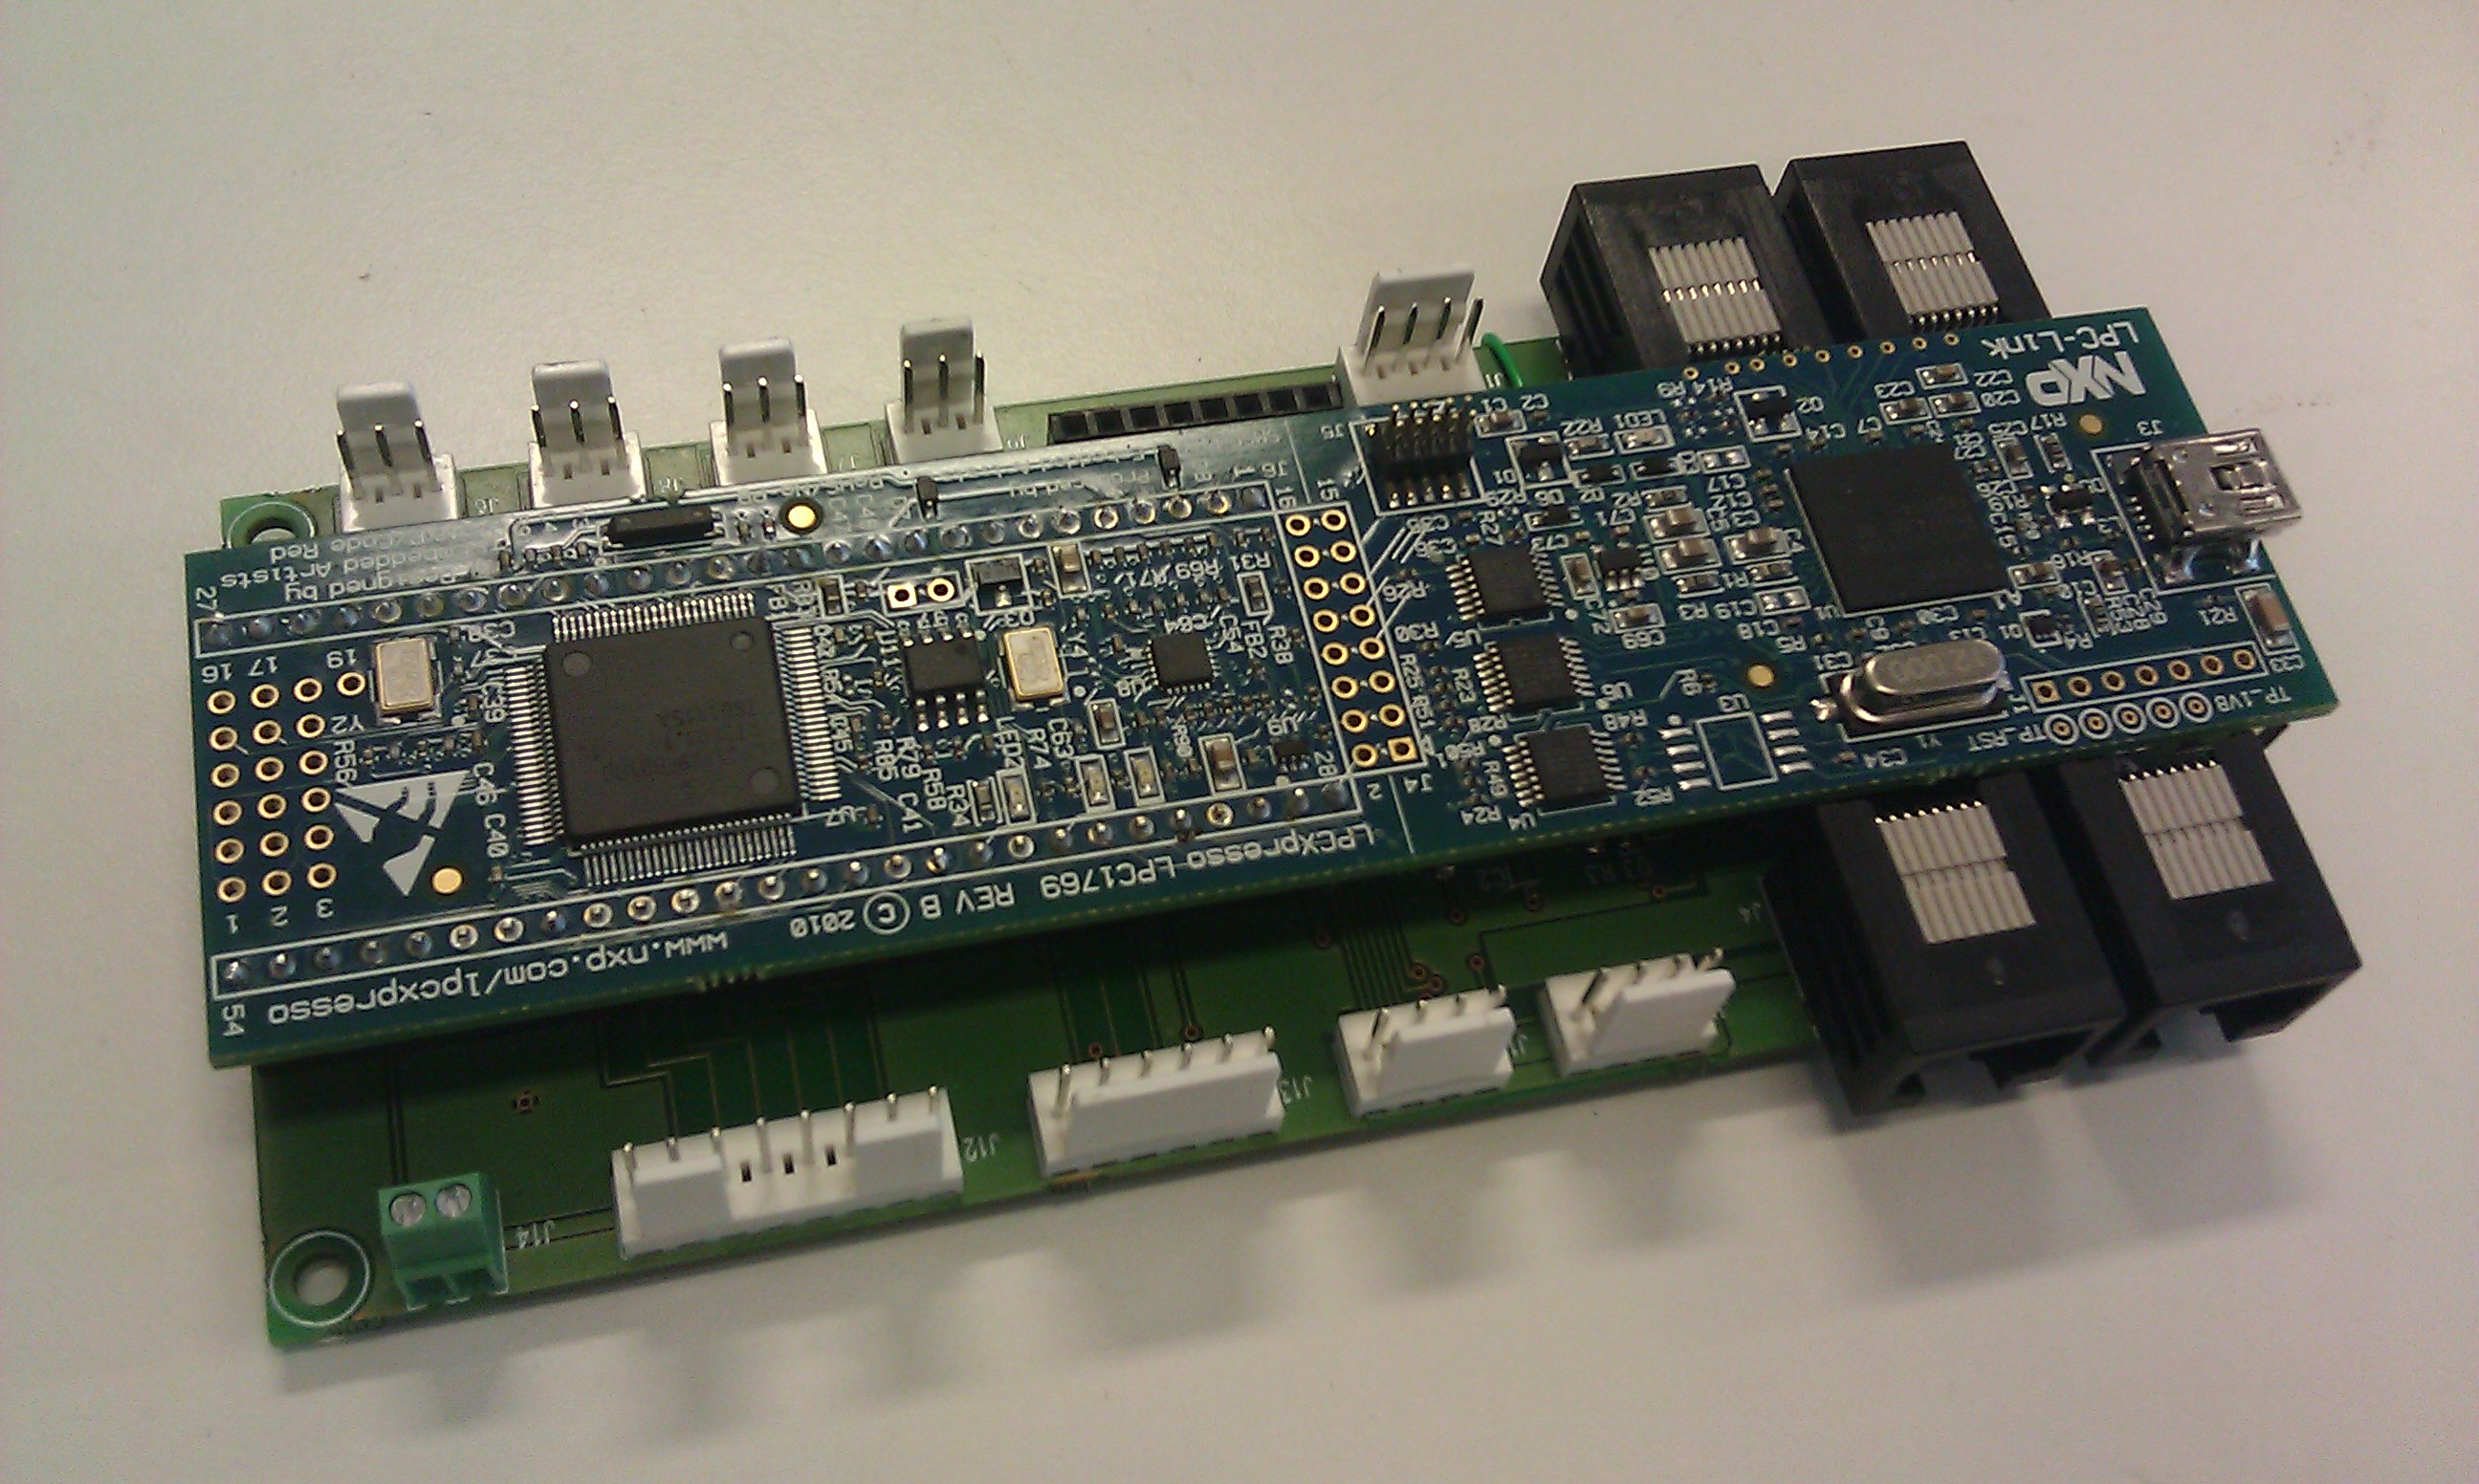
\includegraphics[width=\columnwidth]{LPCXpressoShieldAssembly}
			\caption{The LPCXpresso LPC1769 and the LPCXpresso shield V1 assembly}
			\label{fig:shield}
		\end{figure}
	
	\subsection*{Tools}
		The LPCXpresso platform comes with an IDE.
		This IDE is especially good for debugging code for the LPCXpresso:
		you can set breakpoints and step through the code while visually inspecting all the registers.
		The IDE will be very helpful while developing the CAN bootloader.
		
		The LPCXpresso IDE is free to use for programs that are smaller than 128kB.
		The department however wants to develop for the nodes in a high level language like eLua or proto,
		which means that they want to flash a large image with the virtual machine onto the nodes.
		To circumvent this restriction they utilize the built-in UART bootloader of the LPC1769.
		To work with the UART bootloader they use cables to communicate between the computer and processor over UART.
		These cables can also be used to send debug information between the hostcomputer and the processor.
		We can keep this in mind while developing for the LPC1769.
		
		The department has 2 Saleae Logic's which are logic analyzers.
		With those logic analyzers we can monitor signals in the hardware which is very useful while debugging.
	
	\subsection*{Facilties}
		The faculty has an electronics room with most common equipment like soldering irons, breadboards and jumper wires.
		We can use these as we like for making test setups for the node.

\section*{Design}
	After the orientation project we focussed on the main problem: the CAN bootloader for the LPC1769.
	We tried to do a complete as possible design of the software before starting implementation of the bootloader.
	
	\subsection*{Overview LPC1769}
		The memory of the LPC1769 looks like \autoref{fig:flash}.
		Our program must reside in the Flash memory along with the user program.
		\begin{figure}[htbp]
			\centering
			\begin{bytefield}{24}
				\memsection{0x1000 7FFF}{0x1000 0000}{5}{Local Static RAM}
				\memsection{0x0FFF FFFF}{0x0008 0000}{5}{\textit{reserved}}
				\memsection{0x0007 FFFF}{0x0000 0401}{5}{Flash Memory}
				\memsection{0x0000 0400}{0x0000 0008}{3.2}{Interrupt vector table}
				\memsection{0x0000 0007}{0x0000 0004}{2.2}{Stack pointer}
				\memsection{0x0000 0003}{0x0000 0000}{2.2}{Start pointer}
			\end{bytefield}
			\caption{Relevant parts of the LPC1769 memory}
			\label{fig:flash}
		\end{figure}
		
		The LPC1769 has a lot of built-in peripherals,
		which are hardware functionalities.
		One can interact with these peripherals via registers.
		The CAN peripheral consists of 2 registers, which are needed to be used to perform all functionality.
		Implementing all functionality can be done with interrupts or by polling the registers.
		In the case of polling the registers, it is called a blocking implementation since no other function can be performed by the processor while waiting for something.
	
	\subsection*{Functions and requirements}
		After analysis of what the bootloader was supposed to do we divided the problem in the following functions:
		\begin{itemize}
			\item The bootloader must activate when you want to reprogram the processor via the CAN bus.
			\item One must be able to choose to only program one node on a CAN bus.
			\item The bootloader must download the program (in parts) over the CAN bus to RAM.
			\item The bootloader must copy the downloaded program into the processors flash.
			\item The bootloader must start the newly downloaded program after programming.
		\end{itemize}
		After functional analysis of the problem we identified requirements to within implement the bootloader.
		\begin{itemize}
			\item The bootloader should use as little ROM memory as possible.
			\item The bootloader should be as transparent as possible to the programmer that uses the bootloader. With this requirement we mean that the programmer that is using this bootloader shouldn't have to think about it, he should not notice that there is a bootloader in the ROM where his program also is.
			\item Flashing all nodes in the network should be able to be done in reasonable time.
		\end{itemize}
		
		We will discuss per function how we are planning on implementing different aspects of the bootloader an why we want to do it that way.
	
	\subsection*{Location of the bootloader}
		The bootloader has to be in ROM with the user program, there is no other option.
		For the place of the bootloader we identified two concepts:
		\begin{itemize}
			\item Compiling the bootloader with the user program.
			\item Putting the bootloader at the top of the flash memory and implementing all the peripheral functions polling.
			\item Putting the bootloader at the top of the flash memory and implementing the peripheral functions with interrupts.
		\end{itemize}
		
		\subsubsection*{Compiling in user program}
			In this concept you make a function that the user program should call before executing its own program.
			You still have some slack in this whether you call the bootloader function before or after the startup code of the user application.
			
			We identified some problems with this approach.
			Foremost the bootloader code is somewhere among the user application code,
			which means that the code the bootloader is replacing is also the place where the bootloader code itself is.
			This could be solveed by linking you bootloader code like it is in RAM and then have a piece of code that copies the bootloader to RAM and starts it.
			
			Another problem is that if you accidentally flashes the wrong problem or made a mistake in your program why it does not flash you have bricked the node.
			You will have to go to the physical location of the node and reprogram it via the JTAG or UART bootloader.
			
			The bootloader itself is also not transparent to the user.
			The user application has to change to facilitate the bootloader.
			This makes the bootloader very platform bound and less re-usable.
		
		\subsubsection*{Top of flash polling}
			In this concept we put the bootloader code at the top of the flash.
			We overwrite the start pointer during flashing to point to the bootloader at the top while saving the original start and stack pointer value.
			So the bootloader is called at startup,
			it can then set up everything needed for the bootloading and then start the user application program.
			Every interaction with the peripherals are done via polling.
			So the interrupts are disabled when the bootloader start so that user application interrupts do not fire.
			
			We have also identified some problems with this approach.
			You have to use the CAN bootloader to load your application into flash,
			programming via the JTAG interface or the UART bootloader will overwrite the CAN bootloader.
			
			The program might try to use the memory where the bootloader is programmed in.
			
			If the bootloader runs during the user application the bootloader does not know the settings of the clock and other peripherals.
			The bootloader must also not use RAM that the application uses. 
			
			Since the user application and bootloader are now completely separate you can flash every program you want in the flash.
			
		\subsubsection*{Top of flash interrupts}
			Same as previous but now instead of polling using interrupts.
			To achieve this we must also overwrite the CAN receive interrupt during downloading
	
	\subsection*{Activate the bootloader}
		You need a way to get the processor in bootloader mode while not giving the normal program more constraints.
		The built-in UART bootloader of the LPC1769 activates when during boot a certain pin is pulled low.
		We need to find a way to get nodes in the network to go into our bootloader code when we want to,
		and to keep it in the application code when we just want the application to run.
		
		We generated a few concepts to implement this functionality.
		
		\subsubsection*{Startup message}
			Wait for a certain amount of time during startup and if the node receives a bootloader CAN message go into bootloader mode.
		
		\subsubsection*{Specific CAN message}
			Overwrite the CAN receive interrupt to map to a function in your bootloader.
			Determine if it is a start bootloader message,
			if it is start the bootloader and if it isn't call the user interrupt vector.
			
			This implies that during bootloading you overwrite the user CAN receive interrupt and replace it with your bootloader interrupt.
	
	\subsection*{Downloading to RAM}
		After that the node is in bootloading mode must we be able to get the program to the node over the CAN bus.
		
	
	\subsection*{Flashing the node}
		If we have the program in RAM we must download it into the flash memory.
		In the LPC1769 is an IAP, in application programming, API to perform such tasks with.
		There is a command to copy $x$ number of bytes from RAM to flash.
		Afterwards there is a peripheral to generate a signature of the flashed content.
		With this hash the node can figure out if the flashing was successful or not.
		
		We must take the following constraints into account:
		\begin{itemize}
			\item Interrupts must be disabled or interrupt handlers must reside in RAM during flash programming
			\item You must prepare the sectors you are going to write to with an IAP command before trying to write to it.
		\end{itemize}
	
	\subsection*{Start the program}
		Set the stack pointer and reset the instruction pointer.
		
		Use IAP command GO.
	
	%Linked in application or boot application residing in the top of memory.
	
	%Overriding all interrupts or program bootloader without using interrupts.
	
	%Should we use the CMSIS library functions or write our own drivers.
	
	%Getting the node in bootloader mode.
	
	%IDs for the nodes.
	
	%Tools to program the nodes with, how to facilitate the computer  sensor network interface
	
	\subsection*{Implementation plan}
		While all these features on themselves aren't extremely difficult, debugging these functionalities can be very tedious.
		We think that implementing everything one by one would be easier.
		
		The first step would be to have a compile to bootload in ROM with the bootloader.
		The bootloader must then copy that program to RAM and then flash it to the flash.
		
		After completing the flashing functionality we focus on downloading over the CAN protocol.
		If the node starts up it should already be in bootloader mode.
		What it should do is download the program and flash it.
		
		After getting that functionality working we should get the part that selects if the node should go into bootloading mode working.
		
		If we accomplish all this we should have a functioning CAN bootloader.

\end{document}
